
\documentclass[11pt]{article}

% ---------------- 中文支持（请使用 XeLaTeX 编译） ----------------
\usepackage[UTF8]{ctex}

% ---------------- Packages ----------------
\usepackage[margin=1in]{geometry}
\usepackage{amsmath,amssymb,amsthm}
\usepackage{graphicx}
\usepackage{hyperref}
\usepackage{fancyhdr}
\usepackage{enumitem}
\usepackage{algorithm}
\usepackage{algpseudocode}

% ---------------- Header ----------------
\pagestyle{fancy}
\fancyhf{}
\lhead{Algorithm Design}
\rhead{Homework \#3}
\cfoot{\thepage}
\setlength{\headheight}{14pt}

% ---------------- Title ----------------
\title{Homework 3}
\author{羊瑞 \\ 2300013091}
\date{\today}

% ---------------- Custom commands ----------------
\newcommand{\R}{\mathbb{R}}
\newcommand{\E}{\mathbb{E}}

% ---------------- Problem Environment ----------------
\newcounter{problem}

\newenvironment{problem}[1][]{
\stepcounter{problem}
\section*{Problem \theproblem\; #1}
}{}

\newenvironment{solution}{
\par\noindent\textbf{Solution.}\par\noindent
}{\qed}

\setlength{\parindent}{0pt}

% ---------------- Document ----------------
\begin{document}

\maketitle

% ==================================================
\begin{problem}
\begin{center}
    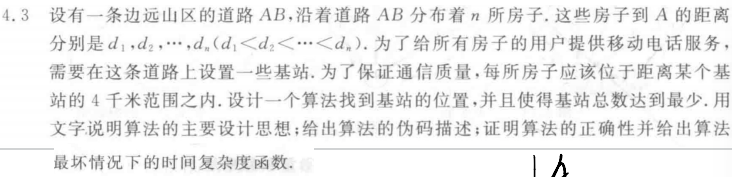
\includegraphics[width=0.6\textwidth]{problems/4.3.png}
\end{center}
\end{problem}

\begin{solution}
若基站设在位置 $x$，则它能覆盖区间 $[x-4,\ x+4] $.

贪心思想：每次先考虑当前最左边尚未被覆盖的房子，记其位置为 $d_i$。为了让这个基站尽可能多地覆盖后面的房子，应当把基站放在该房子能够被覆盖的最靠右位置，即 $x = d_i+4$. 这样它能覆盖区间 $[d_i,\ d_i+8]$,从而尽可能多地覆盖后续房子。然后跳过所有已被该基站覆盖的房子，继续处理下一个未覆盖房子。

\textbf{Algorithm：}
\begin{algorithmic}[1]
\State Input: $d_1<d_2<\cdots<d_n$
\State Output: 基站位置集合 $B$
\State $B\gets \emptyset,\ i\gets 1$
\While{$i\le n$}
    \State $x\gets d_i+4$
    \State $B\gets B\cup\{x\}$
    \While{$i\le n$ and $d_i\le x+4$}
        \State $i\gets i+1$
    \EndWhile
\EndWhile
\State Output $B$
\end{algorithmic}

正确性说明：设当前最左边未覆盖的房子为 $d_i$。任何可行解都必须用某个基站覆盖它，而该基站位置不能超过 $d_i+4$，否则 $d_i$ 将得不到覆盖。  
因此，把该基站放在 $d_i+4$ 是所有可行选择中最靠右的位置，这样不会减少对左端房子的覆盖，同时能使对右侧房子的覆盖范围最大，从而不会比任何其他放法更差。  
于是，贪心地在 $d_i+4$ 处设基站后，问题就转化为对剩余未覆盖房子的同类子问题。故该贪心策略是最优的。

时间复杂度为 $O(n)$.


\end{solution}

% ==================================================
\begin{problem}
\begin{center}
    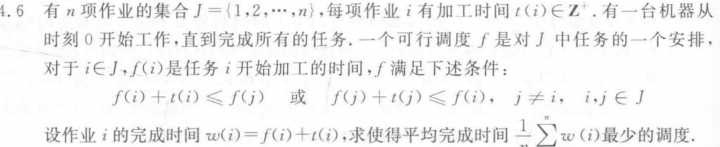
\includegraphics[width=0.6\textwidth]{problems/4.6.png}
\end{center}
\end{problem}

\begin{solution}

设作业 $i$ 的加工时间为 $t(i)$，完成时间为 $ w(i)=f(i)+t(i)$.
目标是最小化平均完成时间$\frac{1}{n}\sum_{i=1}^{n} w(i)$, 而 $n$ 是常数，等价于最小化$\sum_{i=1}^{n} w(i).$

贪心:应当优先安排加工时间短的作业，即按加工时间从小到大排序后依次执行.

\textbf{Algorithm：}
\begin{algorithmic}[1]
\State Input: 作业集合 $J=\{1,2,\dots,n\}$，加工时间 $t(i)$
\State Output: 一个最优调度
\State 按 $t(i)$ 从小到大对所有作业排序
\State 按排序后的顺序依次加工各作业
\end{algorithmic}

正确性说明:设某个调度中有相邻两个作业 $i,j$，并且$t(i)>t(j),$
但调度顺序却是 $i$ 在前、$j$ 在后。设它们之前所有作业的总加工时间为 $T$。

则按顺序 $i,j$ 排列时，这两个作业对总完成时间的贡献为$(T+t(i))+(T+t(i)+t(j))=2T+2t(i)+t(j).$

若交换顺序为 $j,i$，贡献变为$(T+t(j))+(T+t(j)+t(i))=2T+2t(j)+t(i).$

两者之差为$
\bigl(2T+2t(i)+t(j)\bigr)-\bigl(2T+2t(j)+t(i)\bigr)=t(i)-t(j)>0.
$

因此交换后总完成时间变小。  
所以，在最优调度中，不可能存在“较长作业排在较短作业前面”的逆序对。于是最优调度一定是按加工时间非降序排列的。

时间复杂度：$O(nlogn)$.

\end{solution}

% ==================================================
\begin{problem}
\begin{center}
    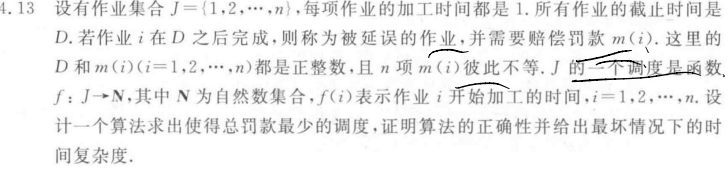
\includegraphics[width=0.6\textwidth]{problems/4.13.png}
\end{center}
\end{problem}

\begin{solution}

由于每个作业长度都相同，若想使总罚款最小，就要在 $D$ 个时段内尽量安排罚款最大的 $D$ 个作业按时完成，其余作业延迟完成。

贪心：按罚款 $m(i)$ 从大到小排序，选出前 $\min\{D,n\}$ 个作业作为“按时完成”的作业集合，其余作业作为迟延作业。  
因为所有按时作业长度都为 $1$，所以只要按任意顺序把这至多 $D$ 个作业安排在时刻 $0,1,\dots,D-1$ 上即可，它们都能在截止时间前完成。

\textbf{Algorithm：}
\begin{algorithmic}[1]
\State Input: 作业集合 $J=\{1,2,\dots,n\}$，共同截止时间 $D$，罚款 $m(i)$
\State Output: 使总罚款最小的调度
\State 按 $m(i)$ 从大到小对作业排序
\State 取前 $\min\{D,n\}$ 个作业组成集合 $A$
\State 其余作业组成集合 $B$
\State 将 $A$ 中作业安排在时刻 $0,1,\dots,|A|-1$
\State 将 $B$ 中作业安排在时刻 $|A|,|A|+1,\dots,n-1$
\end{algorithmic}

正确性说明：由于每个作业加工时间都为 $1$，最多只有 $D$ 个作业能够在截止时间 $D$ 前完成。  
设某个最优解中，按时完成的作业集合为 $A$，迟延作业集合为 $B$。如果存在$i\in A,\quad j\in B,\quad m(j)>m(i),$ 则交换 $i,j$ 的角色：令 $j$ 按时完成、$i$ 迟延完成。交换后总罚款减少了$m(j)-m(i)>0,$
这与原解最优矛盾。  
因此，在任一最优解中，按时完成的必然是罚款最大的那些作业。于是选择罚款最大的前 $D$ 个作业按时完成是最优的。

时间复杂度：$O(nlogn)$.

\end{solution}

% ==================================================
\begin{problem}
\begin{center}
    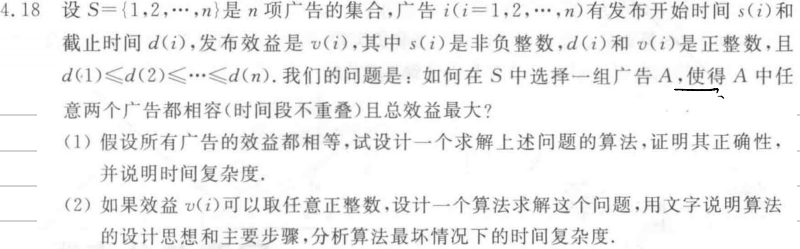
\includegraphics[width=0.6\textwidth]{problems/4.18.png}
\end{center}
\end{problem}

\begin{solution}
每个广告 $i$ 有开始时间 $s(i)$、结束时间 $d(i)$ 和效益 $v(i)$，并且已经满足$d(1)\le d(2)\le\cdots\le d(n).$
(1) 当所有广告效益都相等时
选择尽可能多的互相兼容的广告。  
最优策略是：每次选择当前结束时间最早且与已选广告兼容的广告.

\textbf{Algorithm：}
\begin{algorithmic}[1]
\State 按结束时间从小到大扫描广告
\State 先选第一个广告
\State 之后每次选取开始时间不早于上一个已选广告结束时间的第一个广告
\end{algorithmic}

正确性说明： 结束时间最早的广告为后续广告留下的可用时间最多，因此不会比选择其他广告更差。利用交换论证可证明该贪心算法最优.

时间复杂度：$O(n)$.

\vspace{0.5em}
(2) 当效益 $v(i)$ 可为任意正整数时
先定义 $p(i)=\max\{j<i\mid d(j)\le s(i)\},$
即与广告 $i$ 兼容的、结束时间最晚的广告下标；若不存在，则令 $p(i)=0$。

再定义状态$dp[i]$ 表示只考虑前 $i$ 个广告时可获得的最大总效益。

则递推关系为 $dp[i]=\max\{dp[i-1],\ dp[p(i)]+v(i)\}.$

\begin{itemize}
    \item 不选广告 $i$，则最优值为 $dp[i-1]$；
    \item 选广告 $i$，则其之前只能接一个与之兼容的最优方案，即 $dp[p(i)]$，总效益为 $dp[p(i)]+v(i)$。
\end{itemize}

初始条件: $dp[0] = 0$

最终答案为 $dp[n] $

\textbf{Algorithm：}
\begin{algorithmic}[1]
\State 对每个 $i$ 计算 $p(i)$
\State $dp[0]\gets 0$
\For{$i=1$ to $n$}
    \State $dp[i]\gets \max\{dp[i-1],\ dp[p(i)]+v(i)\}$
\EndFor
\State 输出 $dp[n]$
\end{algorithmic}

正确性说明：对前 $i$ 个广告的最优方案，最后一个广告只有两种可能：选 $i$ 或不选 $i$。  
若不选，则问题退化为前 $i-1$ 个广告的最优解；若选，则前面只能接到 $p(i)$ 为止的最优解。因此状态转移完整且正确。

时间复杂度：对每个 $i$ 用二分查找求 $p(i)$，复杂度为 $O(nlogn) $, 动态规划部分为 $O(n)$.
\end{solution}

% ==================================================
\begin{problem}
\begin{center}
    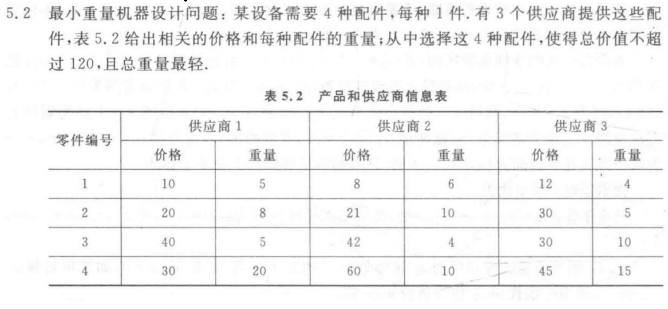
\includegraphics[width=0.6\textwidth]{problems/5.2.png}
\end{center}
\end{problem}

\begin{solution}
设第 $i$ 种配件从第 $j$ 个供应商购买时，价格为 $p_{ij}$，重量为 $w_{ij}$。  
则目标是最小化$ \sum_{i=1}^{4} w_{i,x_i}$并满足$\sum_{i=1}^{4} p_{i,x_i}\le 120,$
其中 $x_i\in\{1,2,3\}$.

由于规模很小，可以直接枚举所有方案，共有81种。逐一计算总价格和总重量，在满足预算约束的前提下取总重量最小者。

根据表中数据, 经枚举可得最优方案为：
\begin{itemize}
    \item 配件 1：选供应商 3，价格 $12$，重量 $4$；
    \item 配件 2：选供应商 1，价格 $20$，重量 $8$；
    \item 配件 3：选供应商 2，价格 $42$，重量 $4$；
    \item 配件 4：选供应商 3，价格 $45$，重量 $15$。
\end{itemize}

于是总价格为$12+20+42+45=119\le 120,$
总重量为
\[
4+8+4+15=31.
\]

因此最优解为：选择(3,1,2,3)号供应商，最小总重量为31.

时间复杂度： 
枚举总数为 $3^4=81$，因此时间复杂度为 $O(3^4)$.
在一般情况下，若有 $n$ 类配件、每类有 $m$ 个供应商，则复杂度为 $O(m^n)$.

\end{solution}

% ==================================================
\begin{problem}
\begin{center}
    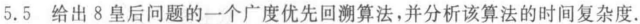
\includegraphics[width=0.6\textwidth]{problems/5.5.png}
\end{center}
\end{problem}

\begin{solution}
按行逐层扩展状态，第 $k$ 层表示前 $k$ 行已经放好了皇后。
状态表示：
用一个长度为 $k$ 的向量$(x_1,x_2,\dots,x_k)$
表示前 $k$ 行的放置情况，其中 $x_i$ 表示第 $i$ 行皇后所在列。

结点扩展规则：
从第 $k$ 层状态扩展到第 $k+1$ 层时，尝试把第 $k+1$ 行皇后放在每一列 $j\in\{1,\dots,8\}$，只保留满足以下条件的位置：
\[
x_i\neq j,\qquad |x_i-j|\neq |i-(k+1)|,\quad i=1,2,\dots,k.
\]

广度优先算法：
\begin{algorithmic}[1]
\State 将空状态入队
\While{队列非空}
    \State 取出队首状态 $(x_1,\dots,x_k)$
    \If{$k=8$}
        \State 输出一个解
    \Else
        \For{$j=1$ to $8$}
            \If{将第 $k+1$ 行皇后放在第 $j$ 列合法}
                \State 将新状态 $(x_1,\dots,x_k,j)$ 入队
            \EndIf
        \EndFor
    \EndIf
\EndWhile
\end{algorithmic}

正确性说明：该算法按层枚举所有可能的部分解，并在每一步利用约束条件剪去不可能扩展成解的状态，因此不会漏掉任何合法解；当扩展到第 $8$ 层时得到的恰好是完整解。

时间复杂度：最坏情况下，每一层最多有 $8$ 个分支，因此状态空间上界为 $O(8^8)$.
考虑到同列冲突的限制，更精确的上界可写成 $O(8!).$

\end{solution}

% ==================================================
\begin{problem}
\begin{center}
    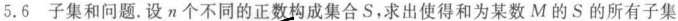
\includegraphics[width=0.6\textwidth]{problems/5.6.png}
\end{center}
\end{problem}

\begin{solution}
状态表示：设当前处理到第 $k$ 个元素，当前已选元素和为 $sum$。

\begin{itemize}
    \item 若 $sum=M$，则得到一个解；
    \item 若 $sum>M$，由于所有数均为正整数，不可能再得到解，立即回溯；
    \item 若 $k>n$ 仍未达到 $M$，则回溯。
\end{itemize}

回溯算法：
\begin{algorithmic}[1]
\Procedure{Backtrack}{$k, sum$}
    \If{$sum=M$}
        \State 输出当前子集
        \State \Return
    \EndIf
    \If{$k>n$ or $sum>M$}
        \State \Return
    \EndIf
    \State 选择 $a_k$
    \State \Call{Backtrack}{$k+1,\,sum+a_k$}
    \State 不选择 $a_k$
    \State \Call{Backtrack}{$k+1,\,sum$}
\EndProcedure
\end{algorithmic}

初始调用为 $\text{Backtrack}(1,0).$

正确性说明：每个元素都被完整地考虑了“选”与“不选”两种情况，因此算法遍历了所有可能子集。由于剪枝仅发生在当前和已超过 $M$ 时，而所有元素都为正，因此这些分支不可能再形成合法解，故剪枝是安全的。

时间复杂度：$O(2^n)$

\end{solution}

% ==================================================
\begin{problem}
\begin{center}
    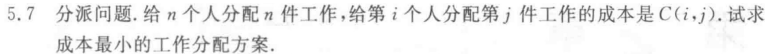
\includegraphics[width=0.6\textwidth]{problems/5.7.png}
\end{center}
\end{problem}

\begin{solution}
状态表示：按人依次分配工作。设当前已经给前 $k-1$ 个人分配了工作，当前成本为 $cost$，并记录哪些工作已被使用。
给第 $k$ 个人尝试分配一个尚未被使用的工作 $j$，然后递归处理第 $k+1$ 个人。  
当 $k=n+1$ 时，说明所有人都完成分配，此时若总成本更小，就更新最优解。

Algorithm：
\begin{algorithmic}[1]
\State $best \gets +\infty$
\Procedure{Backtrack}{$k, cost$}
    \If{$k=n+1$}
        \If{$cost<best$}
            \State $best\gets cost$
            \State 记录当前分配方案
        \EndIf
        \State \Return
    \EndIf
    \For{每个尚未使用的工作 $j$}
        \If{$cost + C(k,j) < best$}
            \State 将工作 $j$ 分给第 $k$ 个人
            \State 标记 $j$ 已使用
            \State \Call{Backtrack}{$k+1,\ cost+C(k,j)$}
            \State 取消标记
        \EndIf
    \EndFor
\EndProcedure
\end{algorithmic}

初始调用为$\text{Backtrack}(1,0).$

正确性说明：该算法枚举了所有可能的一一分配方案。剪枝条件$cost+C(k,j)\ge best$ 表示即使继续向下搜索，当前部分解的总代价也不会优于已知最优解，因此可以安全剪去，不影响最优性。

时间复杂度：$O(n!)$

\end{solution}

\end{document}
```
